\subsection{Аппроксимирующий закон и исходная ЧП}

В ходе выполнения работы было выполнено аппроксимирующее моделирование исходной числовой последовательности с использованием распределения Эрланга с порядком \( k = 2 \).

На рисунке 7 представлена гистограмма для случайных величин, сгенерированных в соответствии с этим законом распределения, а на рисунке 8 — гистограмма распределения частот исходной числовой последовательности.

\begin{figure}[H]
	\centering
	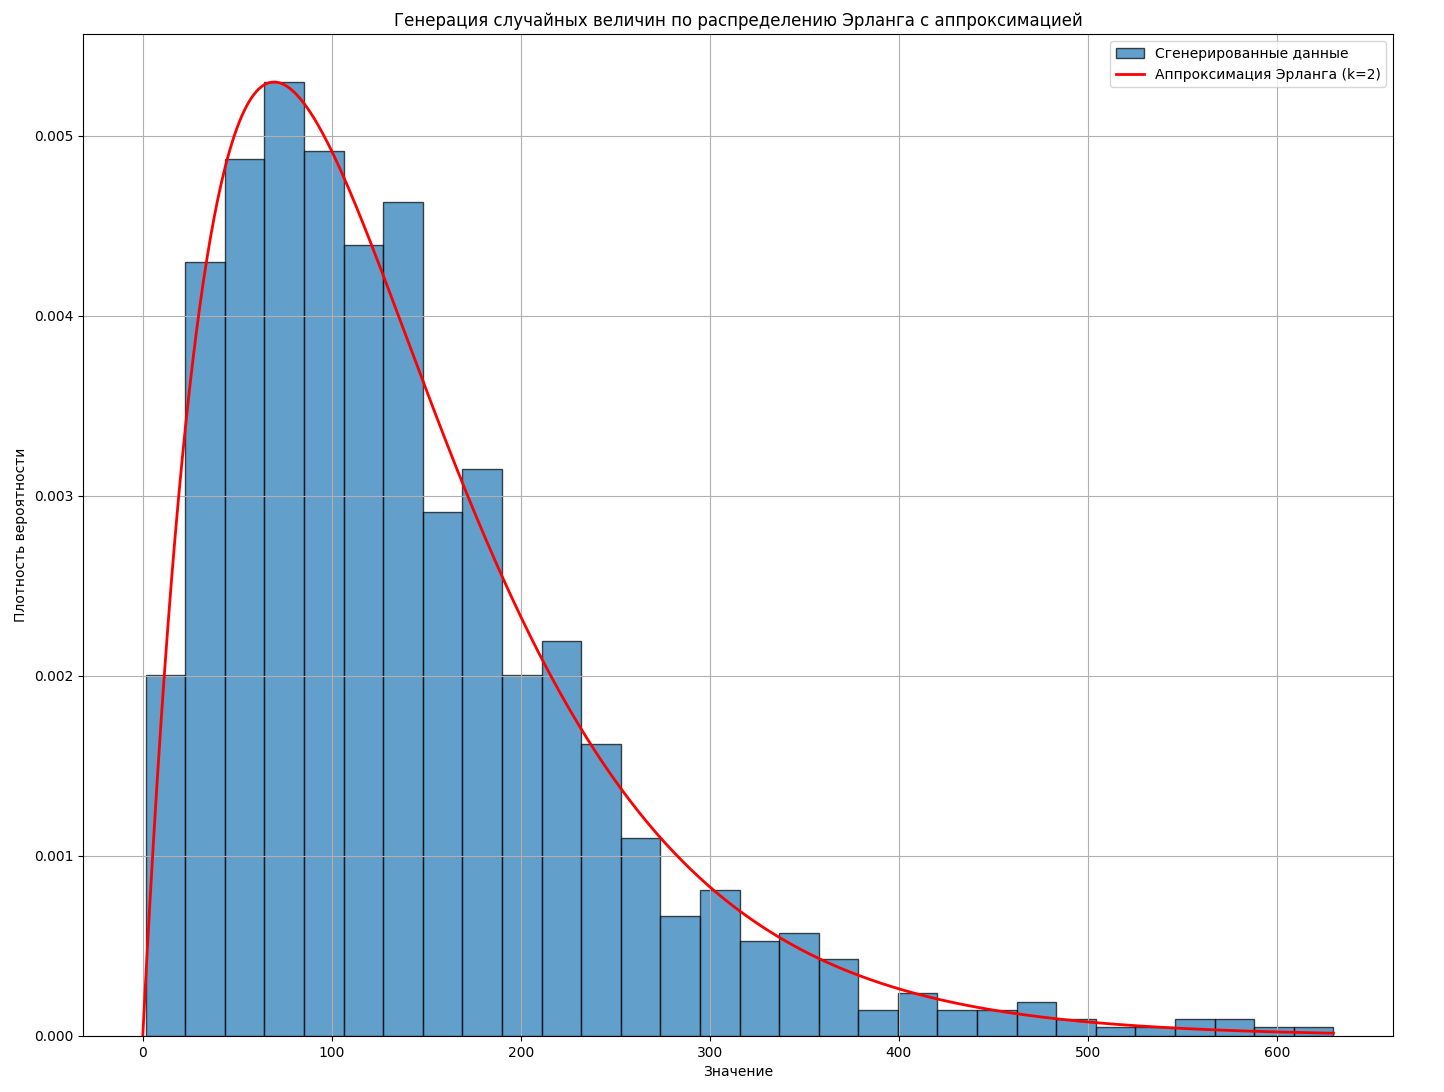
\includegraphics[width=1\textwidth]{../data/histogram_random_generated.png}
	\caption{Распределение Эрланга для сгенерированной последовательности}
\end{figure}

\begin{figure}[H]
	\centering
	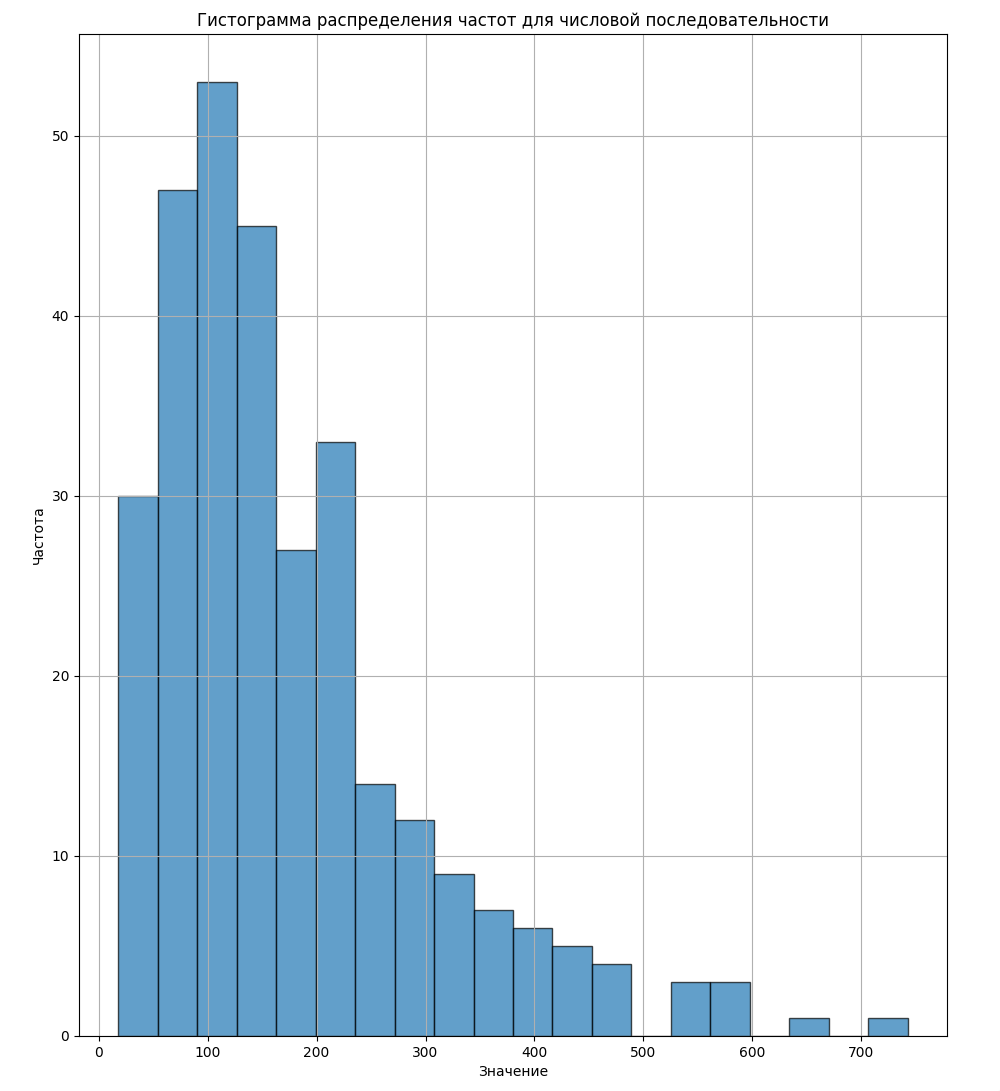
\includegraphics[width=0.8\textwidth]{../data/histogram.png}
	\caption{Гистограмма распределения частот заданной ЧП}
\end{figure}

На основании представленных гистограмм можно сделать вывод, что плотности распределения для сгенерированной по закону Эрланга последовательности и исходной числовой последовательности имеют схожие формы. Гистограммы отображают аналогичное распределение частот, что указывает на правильность выбора аппроксимирующего закона. Несмотря на возможные незначительные отличия в локальных частотах, общая картина подтверждает, что распределение Эрланга хорошо описывает исходную числовую последовательность. Данный результат также подтверждается тем, что коэффициенты вариации и другие числовые характеристики сгенерированных данных находятся в приемлемых пределах отклонений от исходных значений.

\subsection{Форма 2: Таблица числовых моментов для различных выборок}
В таблице ниже представлены числовые моменты для выборок из 10, 20, 50, 100, 200 и 300 значений. Для каждой подвыборки вычислены математическое ожидание, дисперсия, среднеквадратическое отклонение, коэффициент вариации и доверительные интервалы для различных уровней доверия, а также относительные отклонения рассчитанных значений от величин, полученных для выборки из 300 значений.

\FloatBarrier
\begin{table}[H]
	\centering
	\resizebox{\textwidth}{!}{
		\begin{tabular}{|c|c|c|c|c|c|c|c|}
			\hline
			\multirow{2}{*}{\textbf{Характеристика}}   &      & \multicolumn{6}{c|}{\textbf{Количество случайных величин}}                                                                                        \\
			\cline{2-8}
			                                           &      & \textbf{10}                                                & \textbf{20} & \textbf{50} & \textbf{100} & \textbf{200} & \textbf{300}               \\
			\hline
			\multirow{2}{*}{\textbf{Мат. ожидание}}    & Знач & 158.251                                                    & 157.526     & 148.864     & 146.513      & 142.194      & \multirow{2}{*}{141.211}   \\
			\cline{2-7}
			                                           & $\%$ & 12.067\%                                                   & 11.553\%    & 5.420\%     & 3.755\%      & 0.697\%      &                            \\
			\hline
			\multirow{2}{*}{\textbf{Дов. инт. (0.9)}}  & Знач & \pm78.005                                                  & \pm45.096   & \pm24.558   & \pm18.992    & \pm12.609    & \multirow{2}{*}{\pm10.018} \\
			\cline{2-7}
			                                           & $\%$ & 678.670\%                                                  & 350.159\%   & 145.146\%   & 89.579\%     & 25.864\%     &                            \\
			\hline
			\multirow{2}{*}{\textbf{Дов. инт. (0.95)}} & Знач & \pm96.263                                                  & \pm54.586   & \pm29.436   & \pm22.696    & \pm15.046    & \multirow{2}{*}{\pm11.948} \\
			\cline{2-7}
			                                           & $\%$ & 705.661\%                                                  & 356.854\%   & 146.364\%   & 89.948\%     & 25.925\%     &                            \\
			\hline
			\multirow{2}{*}{\textbf{Дов. инт. (0.99)}} & Знач & \pm138.292                                                 & \pm74.613   & \pm39.256   & \pm30.041    & \pm19.844    & \multirow{2}{*}{\pm15.740} \\
			\cline{2-7}
			                                           & $\%$ & 778.624\%                                                  & 374.049\%   & 149.409\%   & 90.862\%     & 26.074\%     &                            \\
			\hline
			\multirow{2}{*}{\textbf{Дисперсия}}        & Знач & 18107.943                                                  & 13603.345   & 10728.201   & 13082.825    & 11643.061    & \multirow{2}{*}{11058.907} \\
			\cline{2-7}
			                                           & $\%$ & 63.741\%                                                   & 23.008\%    & -2.990\%    & 18.301\%     & 5.282\%      &                            \\
			\hline
			\multirow{2}{*}{\textbf{Ср. кв. о.}}       & Знач & 134.566                                                    & 116.633     & 103.577     & 114.380      & 107.903      & \multirow{2}{*}{105.161}   \\
			\cline{2-7}
			                                           & $\%$ & 27.961\%                                                   & 10.909\%    & -1.507\%    & 8.766\%      & 2.607\%      &                            \\
			\hline
			\multirow{2}{*}{\textbf{Коэф. вариации}}   & Знач & 85.033\%                                                   & 74.041\%    & 69.578\%    & 78.068\%     & 75.884\%     & \multirow{2}{*}{74.471\%}  \\
			\cline{2-7}
			                                           & $\%$ & 14.183\%                                                   & -0.578\%    & -6.570\%    & 4.830\%      & 1.897\%      &                            \\
			\hline
		\end{tabular}}
	\caption{Числовые моменты для различных выборок ЧП}
\end{table}
\FloatBarrier


\subsection{Результаты автокорреляционного анализа}

Для оценки случайности последовательности использовалось пороговое значение коэффициента автокорреляции — 0.2. Если автокорреляция на сдвиге превышает это значение, последовательность можно считать неслучайной. Но как видно из талицы и графика, ни одно из значений коэффициентов корелляции для исходной последовательности не превышает даже 0,1 -- исходя из этого можно сделать вывод, что числовая последовательность является случайной.

\begin{table}[H]
	\centering
	\resizebox{\textwidth}{!}{
		\begin{tabular}{|c|c|c|c|c|c|c|c|c|c|c|}
			\hline
			\textbf{Сдвиг ЧП}                     & \textbf{1} & \textbf{2} & \textbf{3} & \textbf{4} & \textbf{5} & \textbf{6} & \textbf{7} & \textbf{8} & \textbf{9} & \textbf{10} \\
			\hline
			\textbf{К-т АК} для сген. \textbf{ЧП} & 0.0185     & 0.0372     & 0.0238     & -0.0298    & 0.0550     & 0.0055     & -0.0226    & 0.0331     & -0.0164    & -0.0055     \\
			\hline
		\end{tabular}
	}
	\caption{Коэф. автокорреляции для сгенерированной ЧП}
\end{table}


\begin{figure}[H]
	\centering
	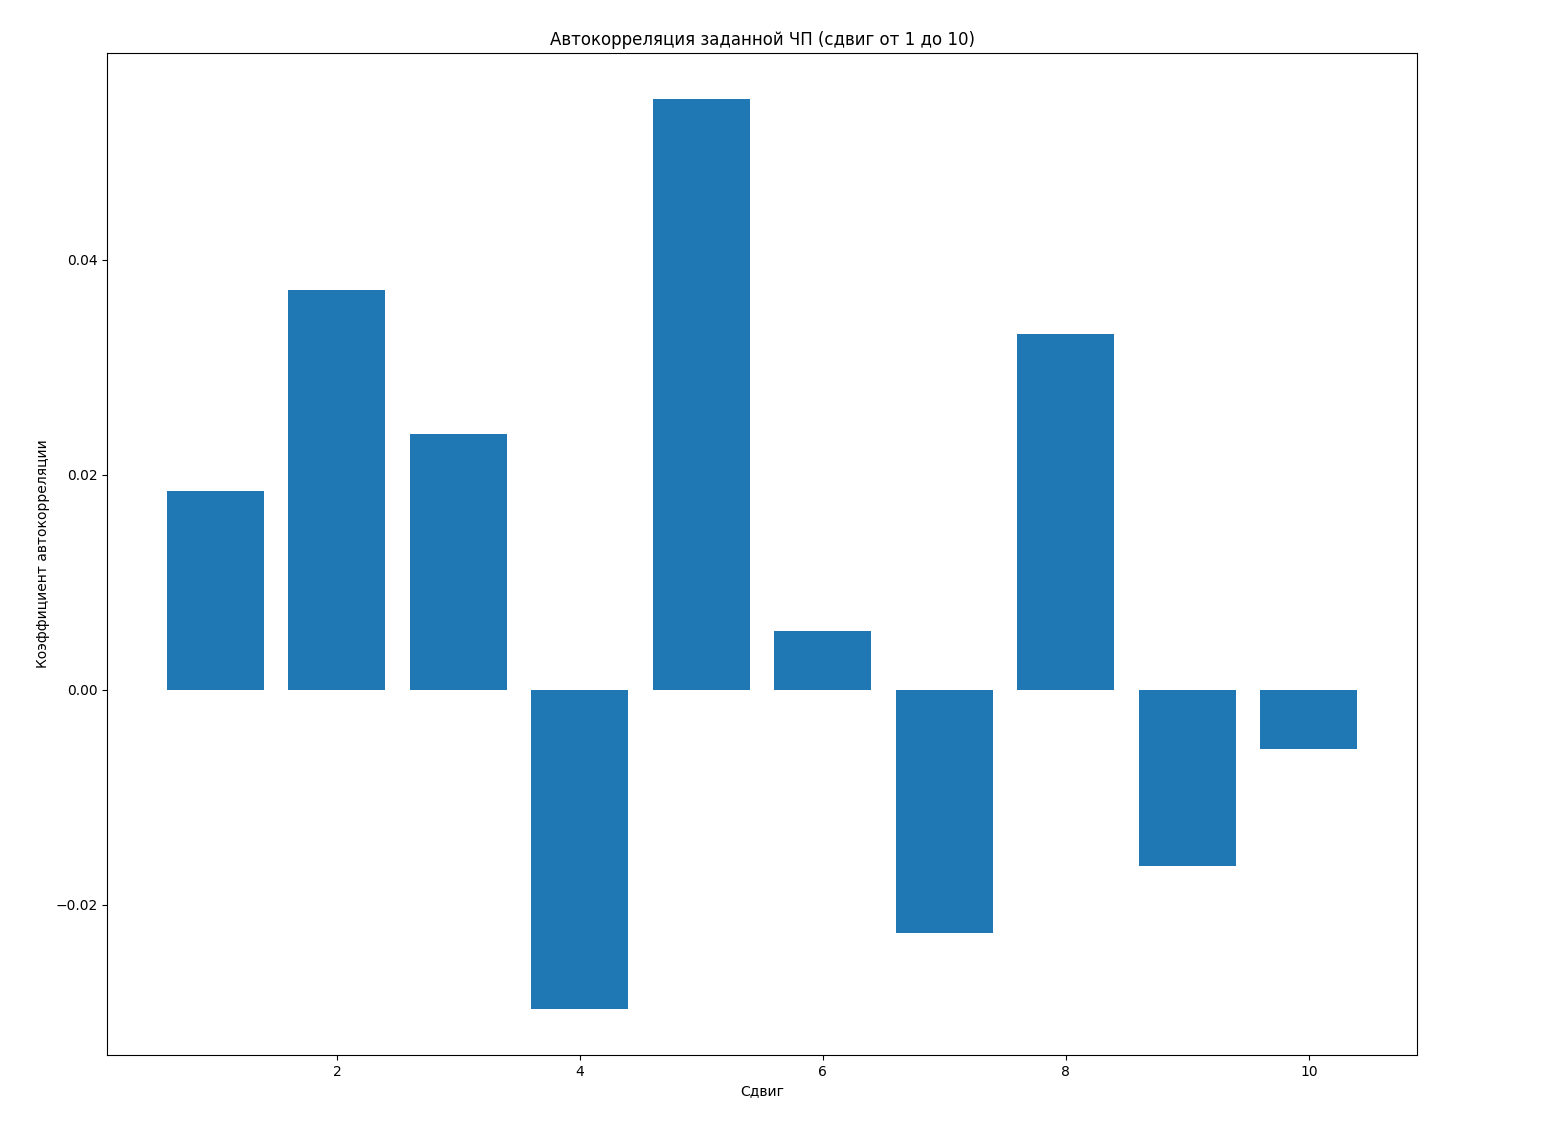
\includegraphics[width=1\textwidth]{../data/auto_corellation_random-2.png}
	\caption{Автокорреляционный анализ для сгенерированной(заданной в этом пункте) числовой последовательности}
\end{figure}

\subsection{Корреляционный анализ}
Для оценки корреляции между сгенерированной последовательностью, полученной с использованием распределения Эрланга, и исходной числовой последовательностью был выполнен корреляционный анализ.

Коэффициент корреляции Пирсона между исходной числовой последовательностью и сгенерированной последовательностью составил:
\[
	r = 0.11363
\]
Этот результат указывает на слабую отрицательную корреляцию, что может свидетельствовать о том, что данные последовательности не имеют сильной линейной зависимости.

Однако такая слабая корреляция не исключает того, что сгенерированная последовательность адекватно моделирует исходную числовую последовательность, поскольку основной упор в аппроксимации делался на плотности распределения, а не на линейной зависимости, а плотность распределения у нас идентична.

На основании полученного коэффициента можно сделать вывод, что аппроксимация исходной последовательности с использованием распределения Эрланга не привела к значительной линейной зависимости между двумя последовательностями, но при этом она точно моделирует эксперимент. Малый коэффициент корелляции лишь означает, что величины в последовательностях независимы, что наоборот хорошо, но не означает, что опыт неточен.

\subsection{Выводы}

\begin{itemize}
	\item В результате проведенного анализа аппроксимации исходной числовой последовательности было установлено, что распределение Эрланга с порядком \( k = 2 \) является подходящим законом распределения для моделирования заданной числовой последовательности. Это подтверждается визуальным сходством гистограммы распределения частот для исходной последовательности и сгенерированной последовательности на основе аппроксимирующего закона.

	\item Расчет числовых характеристик для сгенерированной последовательности, таких как математическое ожидание, дисперсия, среднеквадратическое отклонение и коэффициент вариации, показал, что значения сгенерированных данных находятся в пределах допустимых отклонений от исходных значений. Средние значения и другие статистические моменты подтвердили точность аппроксимации закона распределения.

	\item Автокорреляционный анализ для сгенерированной последовательности показал, что значения коэффициентов автокорреляции не превышают критического порога (0.2), что свидетельствует о случайности последовательности. Этот результат сопоставим с автокорреляционным анализом исходной числовой последовательности, подтверждая, что случайная природа последовательности сохраняется после моделирования.

	\item В целом, выполненные шаги по аппроксимации и сравнению исходной числовой последовательности с сгенерированной в соответствии с законом распределения Эрланга показали высокую степень соответствия, как по визуальным, так и по числовым характеристикам. Таким образом, выбор данного закона для аппроксимации оказался обоснованным и эффективным.
\end{itemize}
